\documentclass{beamer}

\usepackage{graphicx}
\usepackage{mathtools}
\usepackage{mathrsfs}
\usepackage{fdsymbol}
\usepackage{hyperref}

%Information to be included in the title page:
\title{Learning Multivariate Causal Models}
\author{Congyuan Duan}
%\institute{School of Mathematics, Sun Yat-sen University}



\begin{document}

\frame{\titlepage}

\begin{frame}
    \frametitle{Contents}
    \tableofcontents
\end{frame}

\section{Structure Identifiability}

\begin{frame}
    \frametitle{Contents}
    \tableofcontents[currentsection]
\end{frame}

\begin{frame}
    \frametitle{Non-uniqueness of graph structures}
    \begin{flushleft}
        Given a distribution $P_X$ over random variables $X=(X_1,\cdots,X_d)$, there is an SCM
        that induces the distribution $P_X$.  
    \end{flushleft} 
    \centering{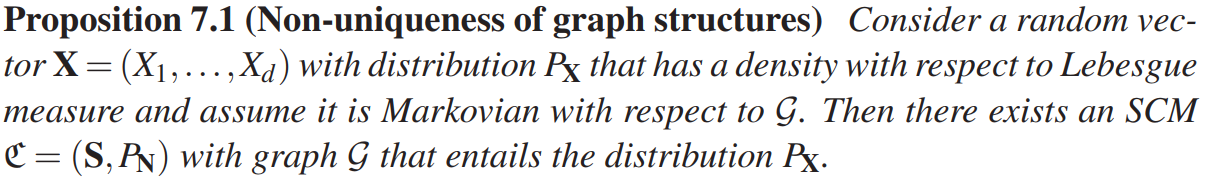
\includegraphics[scale=0.6]{fig1.png}}
    \begin{flushleft}
        In particular, given any complete DAG, we can find a corresponding SCM that
        entails the distribution at hand.
    \end{flushleft}
\end{frame}

\begin{frame}
    \frametitle{Identifiability of Markov equivalence class}
    \begin{flushleft}
        Under the Markov condition and faithfulness, the Markov equivalence class of $\mathcal{G}_0$, 
        represented by $CPDAG(\mathcal{G}_0)$, is identifiable from $P_X$. 
    \end{flushleft} 
    \centering{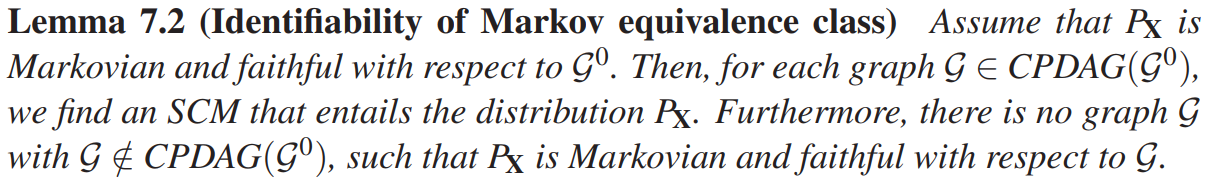
\includegraphics[scale=0.6]{fig2.png}}
    \begin{flushleft}
        However, we are not able to distinguish between two Markov equivalent graphs.
    \end{flushleft}
\end{frame}

\begin{frame}
    \frametitle{Additive Noise Models}
    \begin{flushleft}
        We can restrict the function class to obtain non-trivial identifiability results.
    \end{flushleft} 
    \centering{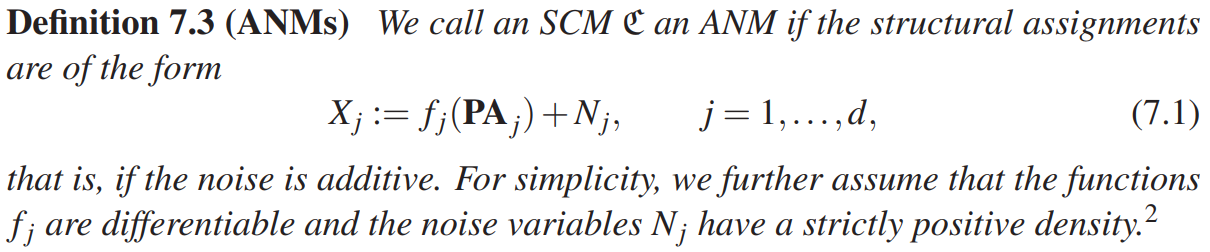
\includegraphics[scale=0.6]{fig3.png}}
    \begin{flushleft}
        Not all restricted class of SCMs described above can obtain full structure identifiability.
    \end{flushleft} 
    \centering{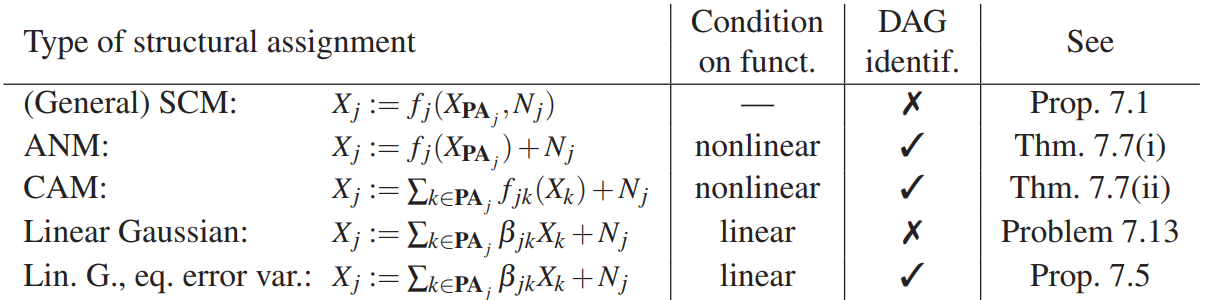
\includegraphics[scale=0.6]{fig5.png}}
    %补一些文字
\end{frame}

\begin{frame}
    \frametitle{Linear Gaussian Models with Equal Error Variances}
    \centering{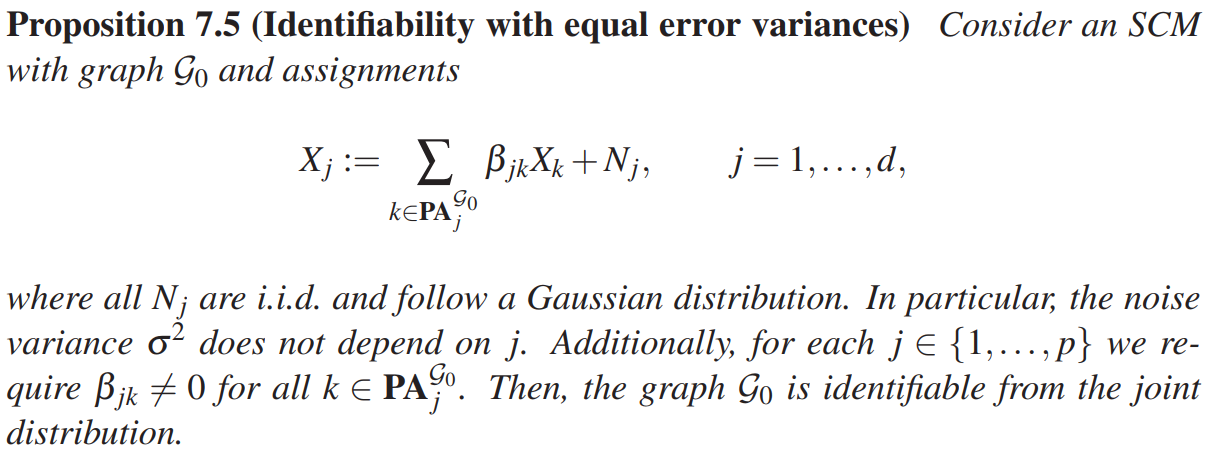
\includegraphics[scale=0.6]{fig6.png}}
\end{frame}

\begin{frame}
    \frametitle{Linear Non-Gaussian Acyclic Models}
    \centering{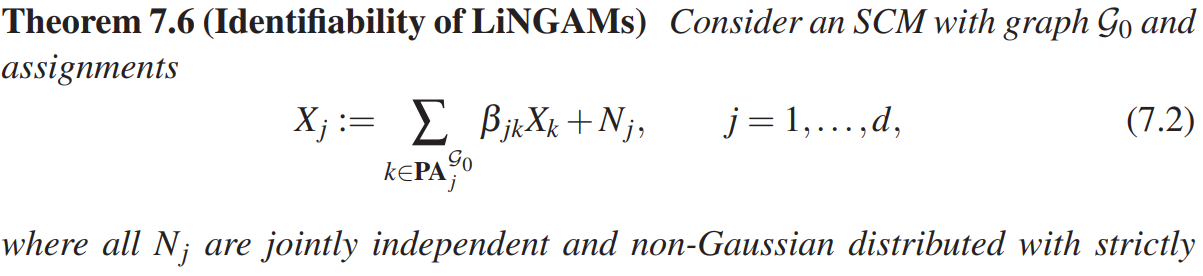
\includegraphics[scale=0.6]{fig7.png}}
    \centering{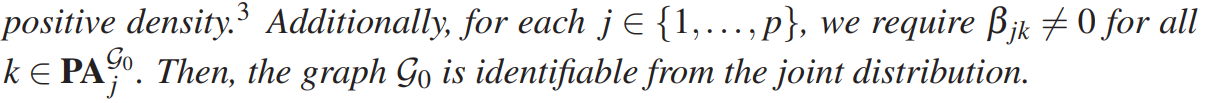
\includegraphics[scale=0.6]{fig8.png}}
\end{frame}

\begin{frame}
    \frametitle{Nonlinear Gaussian Additive Noise Models}
    \centering{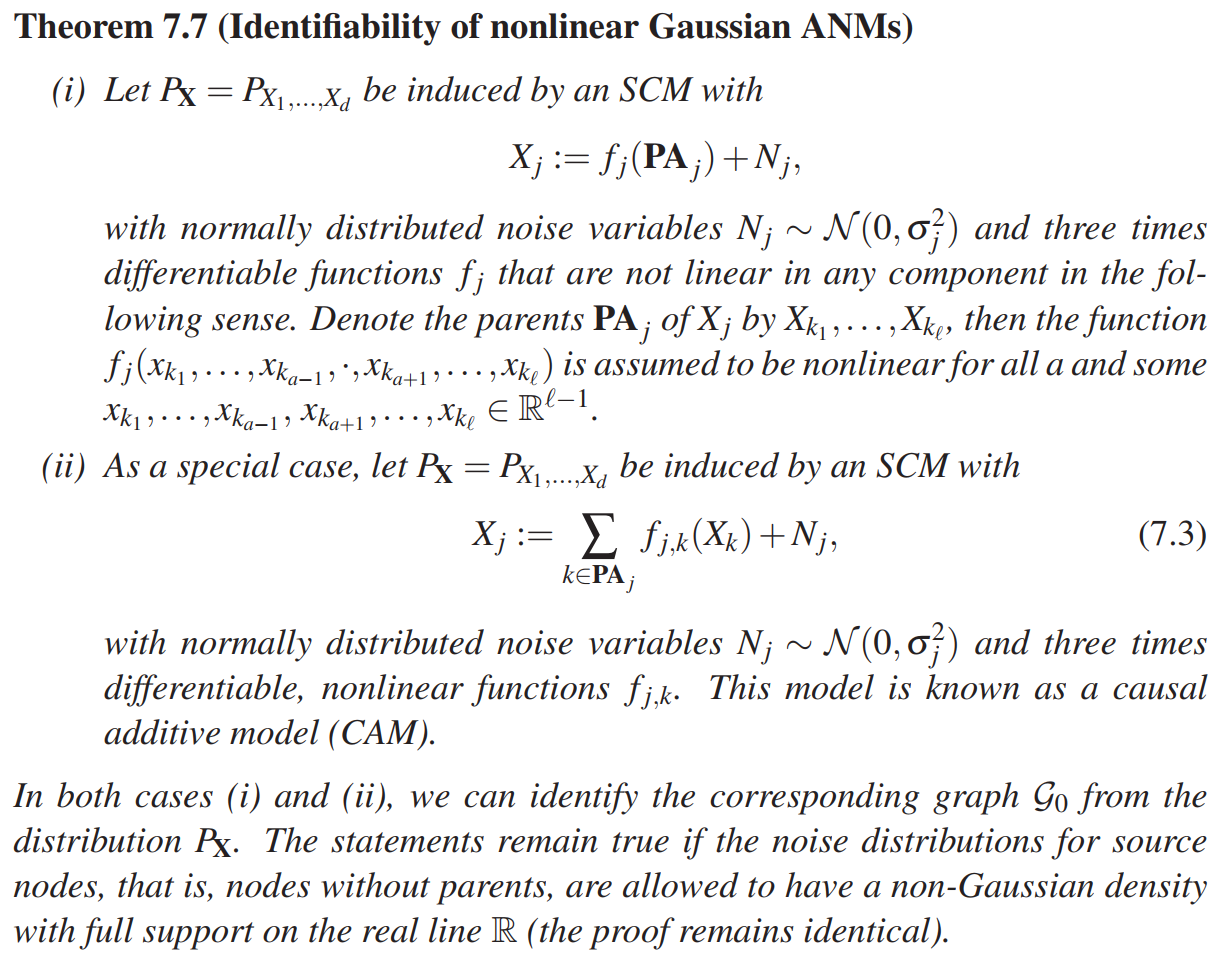
\includegraphics[scale=0.6]{fig9.png}}
\end{frame}

\section{Methods for Structure Identification}

\begin{frame}
    \frametitle{Contents}
    \tableofcontents[currentsection]
\end{frame}

\begin{frame}
    \frametitle{Overview}
    \begin{itemize}
        \item[$\bullet$] \textbf{Independence-Based Methods:} inductive causation (IC) algorithm, PC algorithm \\
        \emph{Independence-based methods assume that the distribution is faithful to the underlying DAG. There is a one-to-one 
        correspondence between d-separations in the graph and conditional independences in $P_X$.}
    \end{itemize}
    \begin{itemize}
        \item[$\bullet$] \textbf{Score-Based Methods:} additive noise models
    \end{itemize}
    \centering{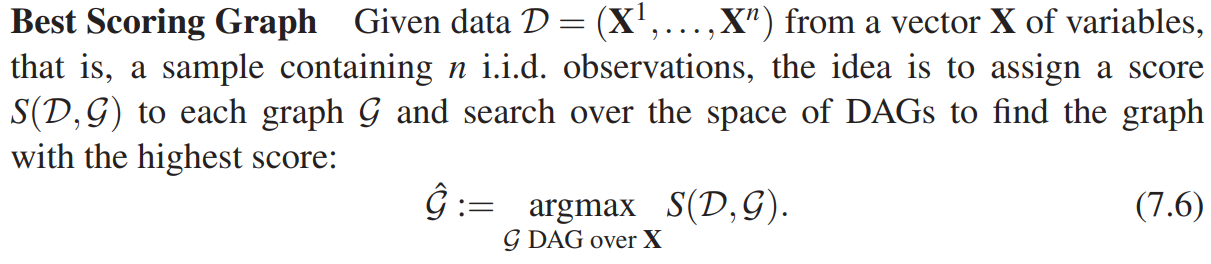
\includegraphics[scale=0.6]{fig11.png}}
\end{frame}

\begin{frame}
    \frametitle{Overview}
    \centering{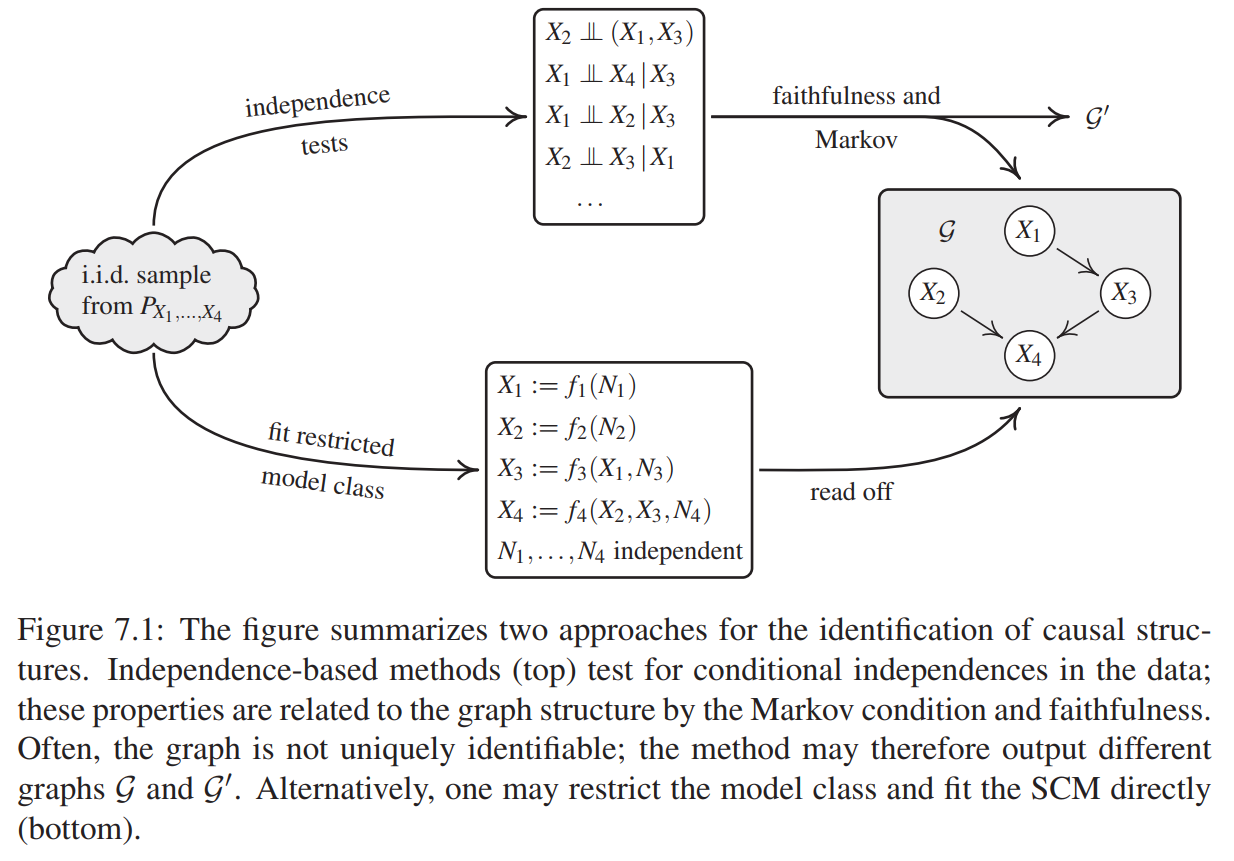
\includegraphics[scale=0.6]{fig10.png}}
\end{frame}

\begin{frame}
    \frametitle{Independence-Based Methods}
    \begin{flushleft}
        Most independence-based methods first estimate the skeleton, that is, the undirected edges, 
        and orient as many edges as possible afterward.
    \end{flushleft}
    \centering{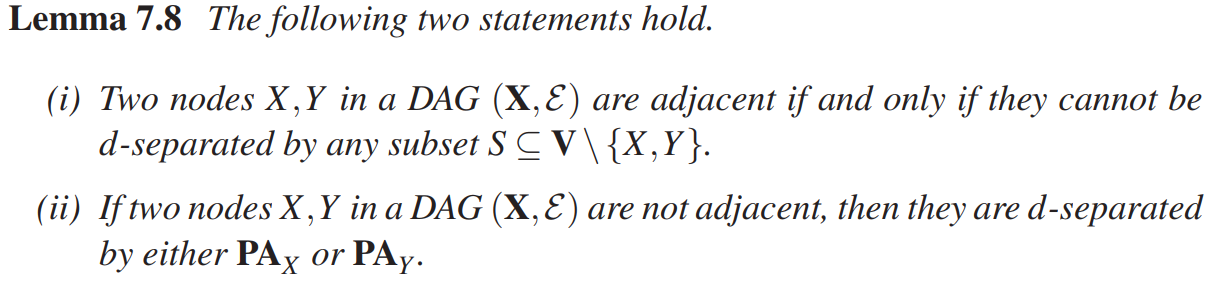
\includegraphics[scale=0.6]{fig12.png}}
    \begin{flushleft}
        We should be able to orient the v-structures in the graph. Suppose that
        the skeleton contains the structure $X-Z-Y$ with no direct edge between X and
        Y; further, let $A$ be a set that d-separates $X$ and $Y$. The structure is
        a v-structure if and only if $Z\notin A$.
    \end{flushleft}
\end{frame}

\begin{frame}
    \frametitle{IC algorithm}
    Abstractly, the algorithm works as follows:
    \begin{itemize}
        \item[$\bullet$] Start with a complete undirected graph on all variables.
        \item[$\bullet$] For each pair of variables, see if conditioning on some set of variables
        makes them conditionally independent; if so, remove their edge.
        \item[$\bullet$] Identify all colliders by checking for conditional dependence; orient the
        edges of colliders.
        \item[$\bullet$] Try to orient undirected edges by consistency with already-oriented edges;
        do this recursively until no more edges can be oriented.           
    \end{itemize}
    %\centering{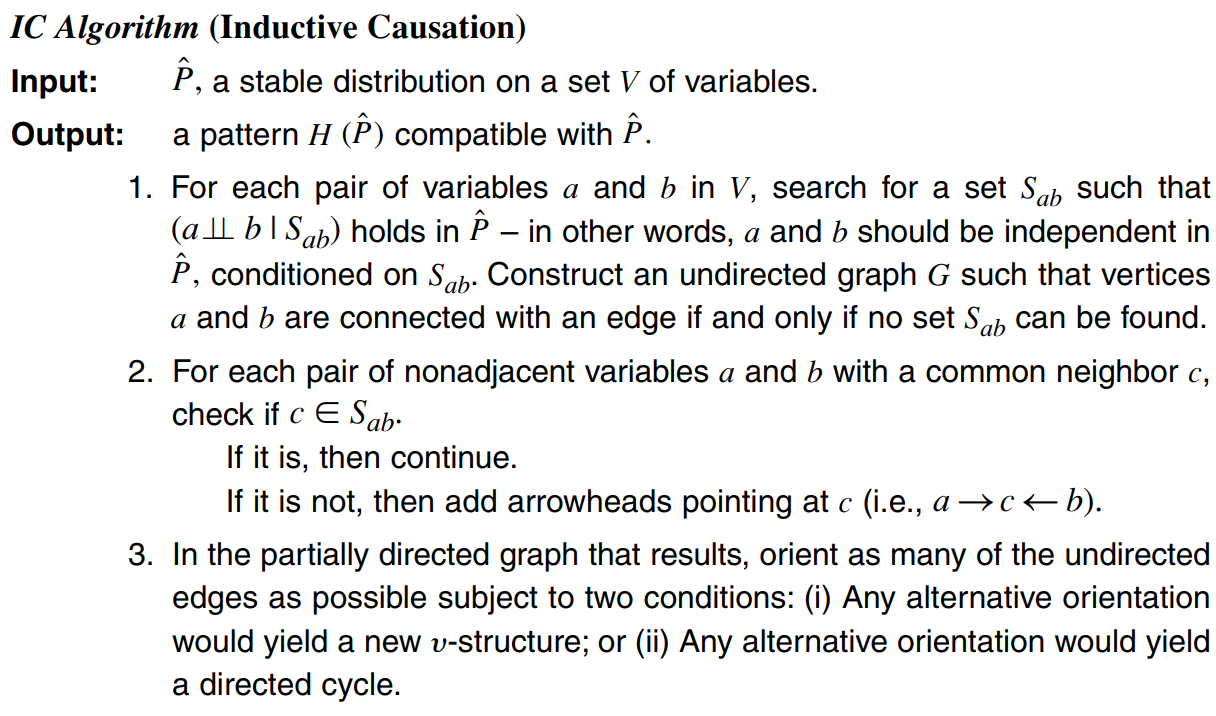
\includegraphics[scale=0.6]{fig20.png}}
\end{frame}

\begin{frame}
    \frametitle{IC algorithm}
    \begin{flushleft}
        In the last step, the following four rules are required for obtaining a maximally oriented pattern.
    \end{flushleft}
    \centering{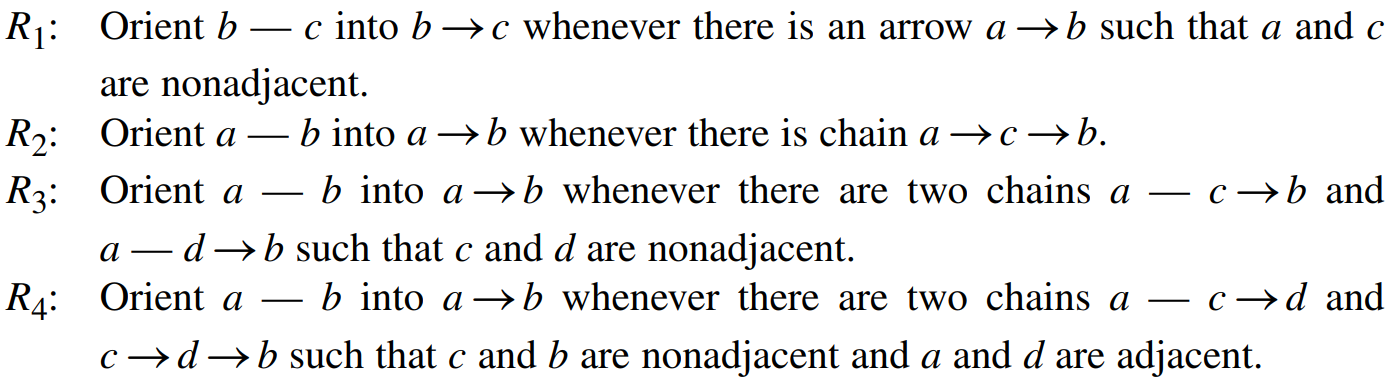
\includegraphics[scale=0.55]{fig13.png}}
\end{frame}

\begin{frame}
    \frametitle{PC algorithm}
    \begin{flushleft}
        Searching through all possible subsets $A$ does not seem optimal, especially if
        the graph is sparse. The PC algorithm step-by-step increases the size of the conditioning
        set $A$.
    \end{flushleft}
    \centering{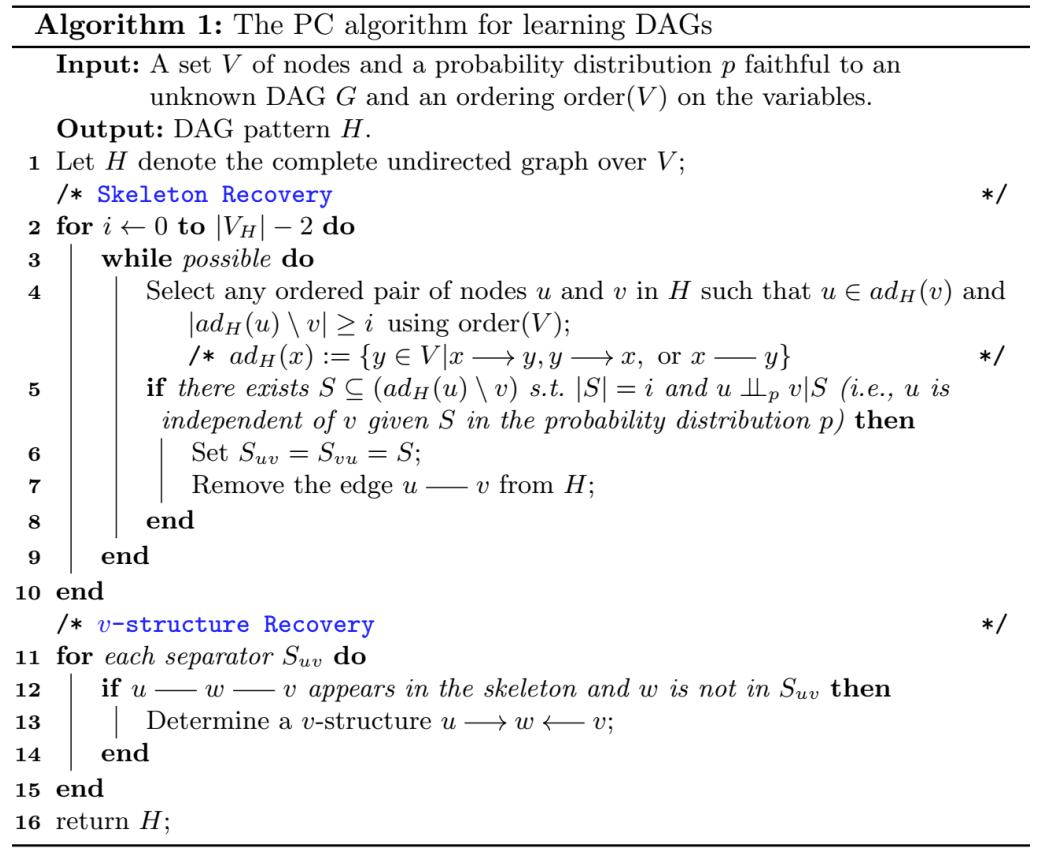
\includegraphics[scale=0.6]{fig18.png}}
\end{frame}

\begin{frame}
    \frametitle{PC algorithm: example}
    \begin{flushleft}
        Obtained conditional independence tests: $B\Vbar C|A$, $A\Vbar D|(B,C)$. \\
        Start with the fully connected undirected graph 
    \end{flushleft}
    \centering{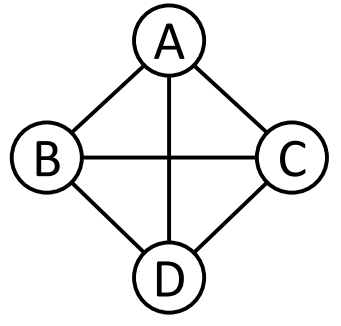
\includegraphics[scale=0.6]{fig15.png}}
    \begin{flushleft}
        After $i=1$
    \end{flushleft}
    \centering{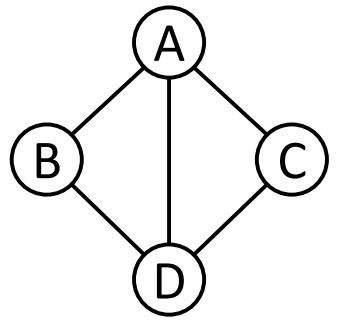
\includegraphics[scale=0.6]{fig16.png}}
\end{frame}

\begin{frame}
    \frametitle{PC algorithm: example}
    \begin{flushleft}
        After $i=2$
    \end{flushleft}
    \centering{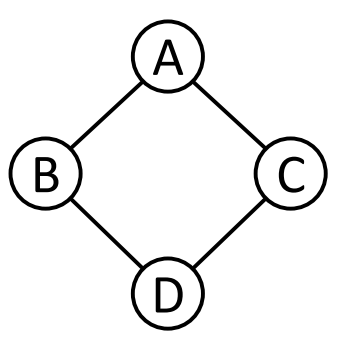
\includegraphics[scale=0.6]{fig17.png}}
    \begin{flushleft}
        v-structure recovery
    \end{flushleft}
    \centering{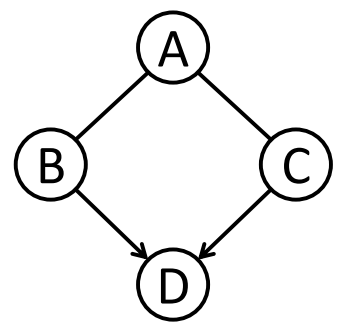
\includegraphics[scale=0.6]{fig19.png}}
\end{frame}

\begin{frame}
    \frametitle{Score-Based Methods}
    \begin{itemize}
        \item[$\bullet$] \textbf{Score Function:} In the nonlinear Gaussian case, for a given graph structure $\mathcal{G}$, 
        we regress each variable on its parents and obtain the score
        \begin{align*}
            &S(\mathcal{D},\mathcal{G}):=\log p(\mathcal{D}|\hat{\theta},\mathcal{G}) - \frac{\#parameters}{2}\log n \\
            &\log p(\mathcal{D}|\mathcal{G})=\sum_j^d -\log \widehat{var}[R_j]
        \end{align*}
        here, $\widehat{var}[R_j]$ is the empirical variance of the residuals $R_j$ obtained from the regression of 
        variable $X_j$ on its parents. 
        \item[$\bullet$] \textbf{Greedy Search Techniques:} At each step there is a candidate graph and a set of
        neighboring graphs. For all these neighbors, one computes the score and considers
        the best-scoring graph as the new candidate. If none of the neighbors obtains a
        better score, the search procedure terminates.  
    \end{itemize}
\end{frame}

\begin{frame}
    \frametitle{Reference} 
    Pearl J. Causality[M]. Cambridge university press, 2009. \\
    https://www.stat.cmu.edu/~cshalizi/402/lectures \\
    https://pooyanjamshidi.github.io/csce580/lectures/ \\
\end{frame}


\end{document}
